%%%%%%%%%%%%%%%%%%%%%%%%%%%%%%%%%%%%%%%%%%%%%%%%%%%%%%%%%%%%%%%%%%% 
%% Desarrollo -  Verificación
%%%%%%%%%%%%%%%%%%%%%%%%%%%%%%%%%%%%%%%%%%%%%%%%%%%%%%%%%%%%%%%%%%%

\subsection{Verificación}
\begin{frame}
  \frametitle{\textbf{Tabla de Contenidos}}
  \begin{center}
    {\vspace{-1.5cm}\Large \textbf{Sección \thesection: \secname }\vspace{0.5cm}}
    \begin{beamercolorbox}[
      sep=8pt,center]{part title}
      \usebeamerfont{part title}
      \textbf{\subsecname}
    \end{beamercolorbox}
  \end{center}
\end{frame}


\begin{frame}
  \frametitle{\textbf{\textbf{Plataforma de verificación}}}
     \framesubtitle{\secname : \subsecname}
    \vspace{-0.3cm}
  \begin{figure}[!t] \centering
  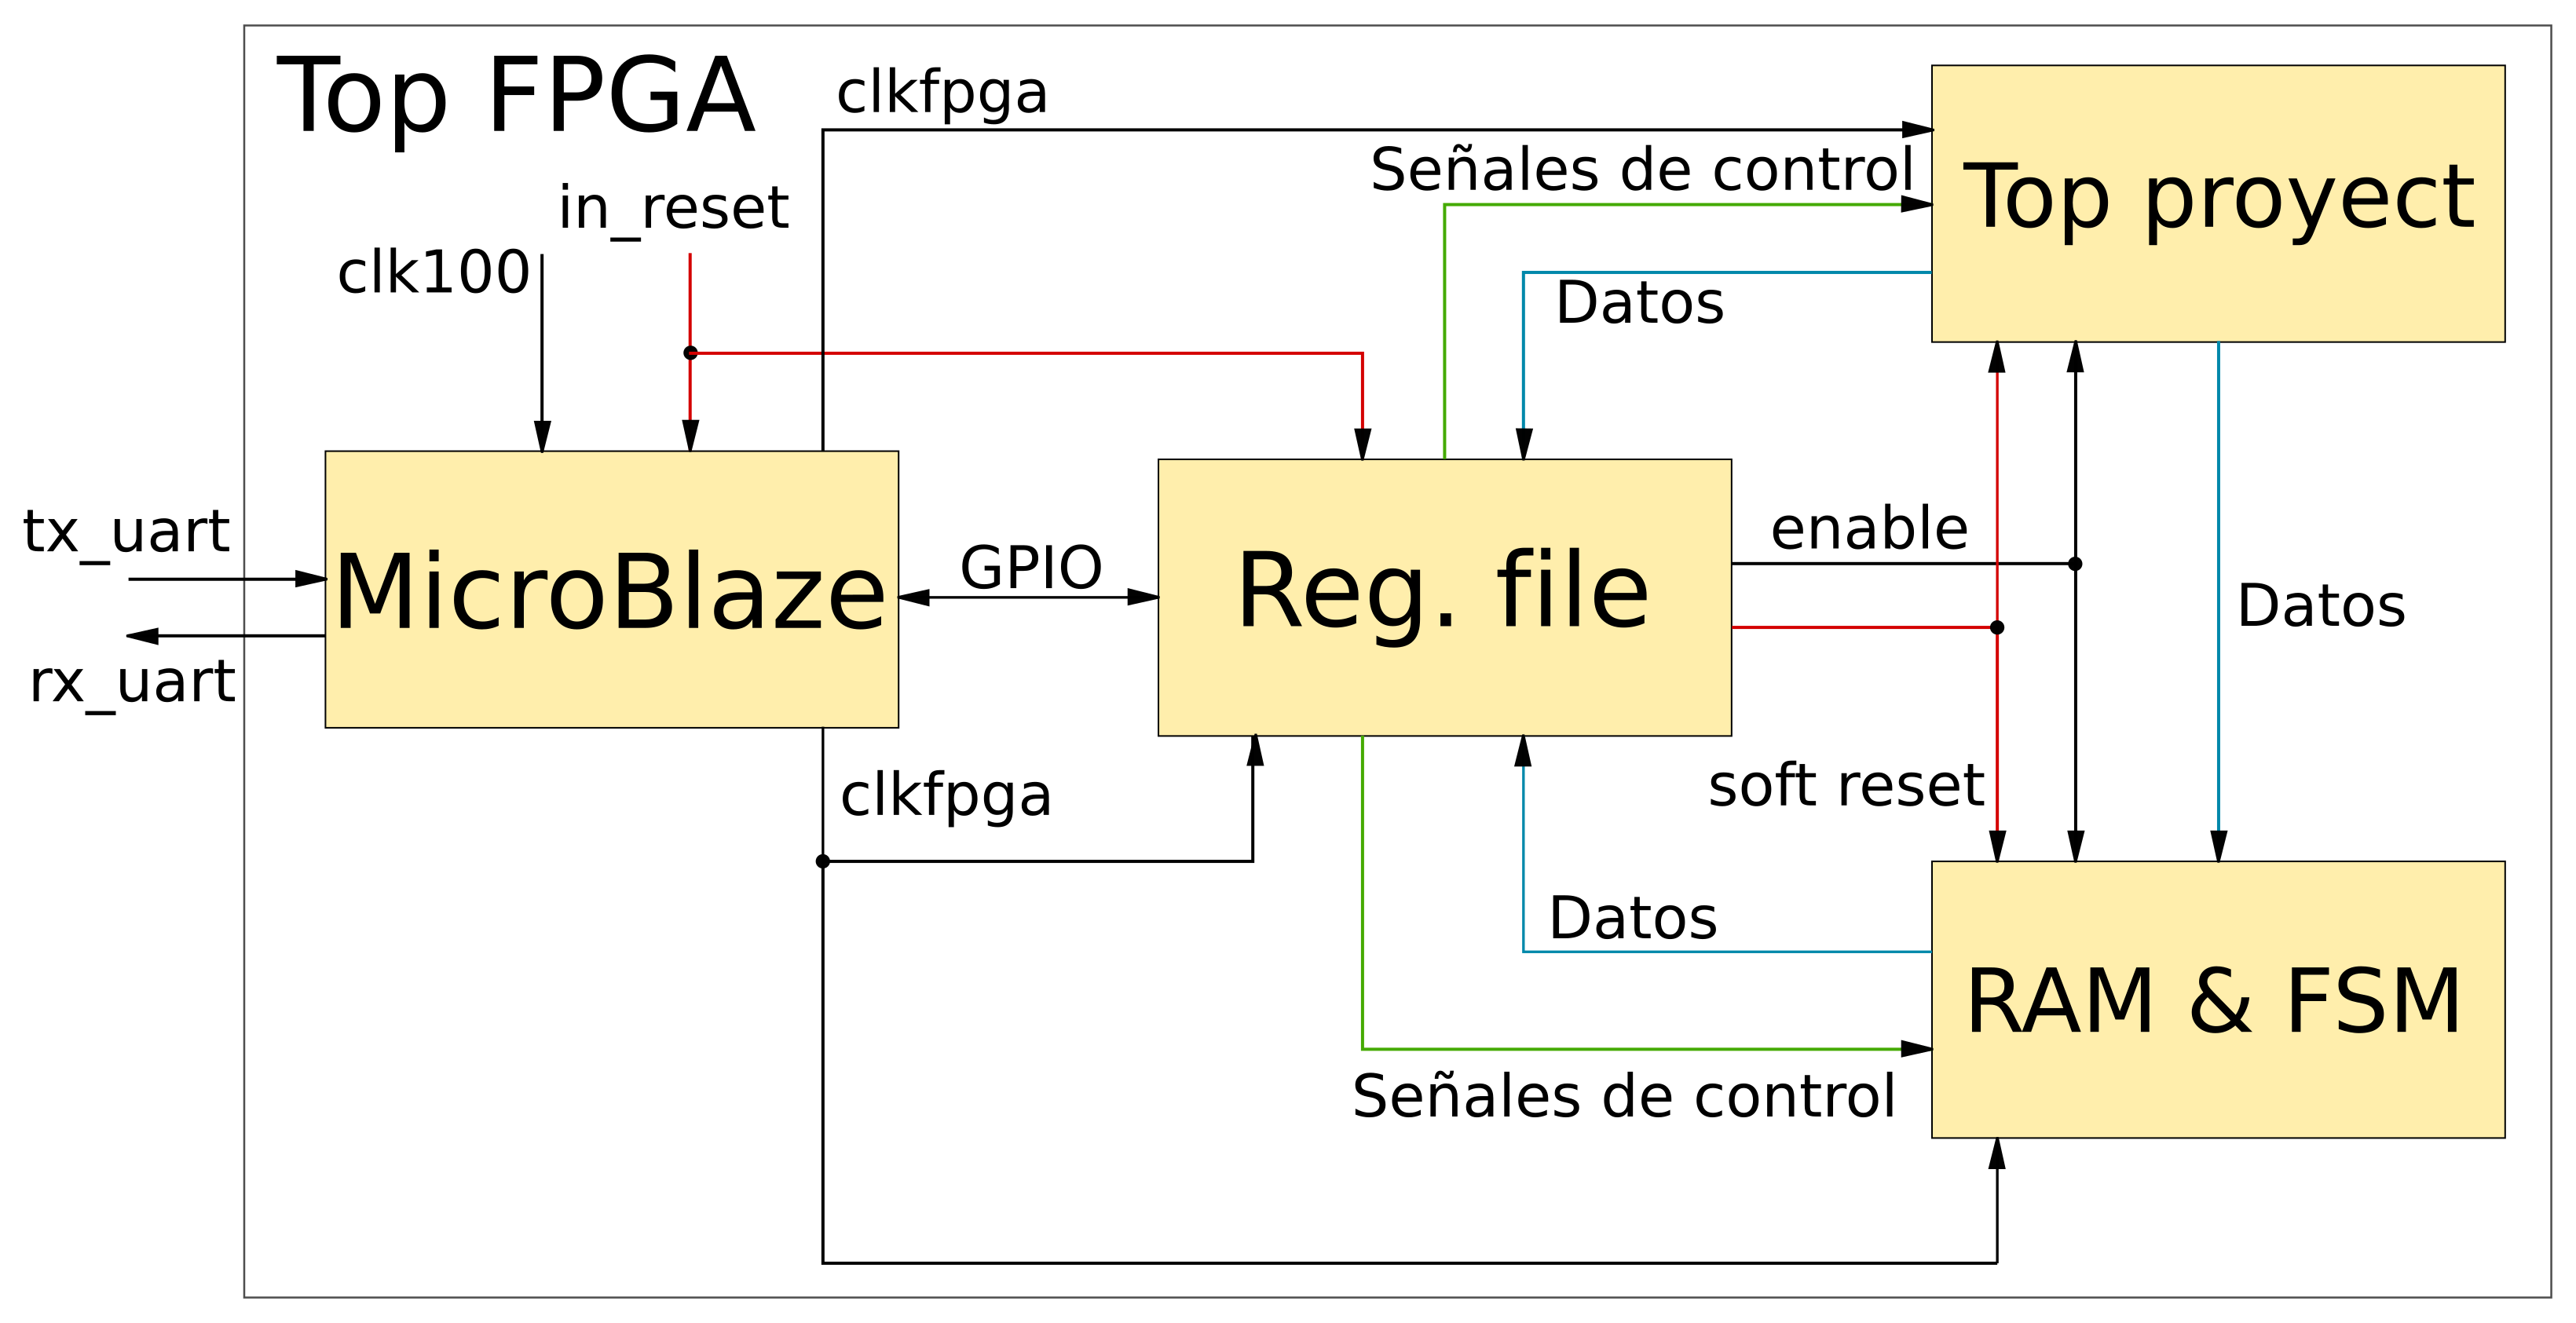
\includegraphics[ width=0.85\paperwidth]{Diagramas/internal_fpga.png}%
  \end{figure}
\end{frame}


% \begin{frame}
%   \frametitle{\textbf{\textbf{Bloques perifericos}}}
%      \framesubtitle{\secname : \subsecname}

%     \begin{block}{\centering \textbf{Generador de bits pseudoaletorios (PRBS)} }
%     \begin{itemize}\small
%         \item Para generar una modulación PAM-4 se utilizan dos PRBS. Una genera el bit de signo mientras y la otra el de magnitud. 
%     \end{itemize}
%     \end{block}
%     \begin{block}{\centering \textbf{Modulo BER}}
%         Consta de dos etapas:
%         \begin{enumerate}\small
%             \item Sincroniza la secuencia de datos decodificada con la secuencia proveniente de la PRBS
%             \item  Dos contadores de 64 bits almacenan la cantidad de muestras de entrada y de errores
%         \end{enumerate}
%     \end{block}
%     \begin{block}{\centering \textbf{Generador de ruido gaussiano (GNG)}}
%         \begin{itemize}\small
%     \item Permite medir niveles de BER extremadamente bajos (~$10^{-15}$). \item El mismo fue obtenido de \cite{gng}. 
%     \end{itemize}
%     \end{block}
% \end{frame}


\begin{frame}
  \frametitle{\textbf{Resultados obtenidos}}
   \framesubtitle{\secname : \subsecname}
   Símbolos codificados, $P_{(x=0)}=0.75$
    \vspace{-0.3cm}

\begin{columns}
    \begin{column}{0.48\linewidth}  
    \begin{figure}
        \centering
    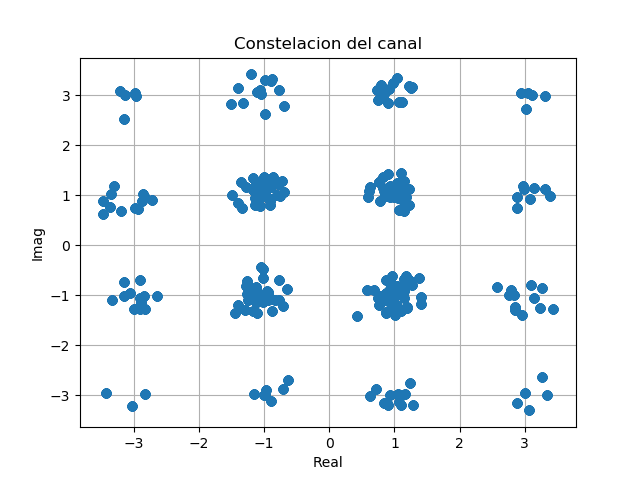
\includegraphics[width=\textwidth]{Graficos/Channel_Constelation.png}%
    \end{figure}
    \end{column}

    \begin{column}{0.48\linewidth}
    \begin{figure}
        \centering
    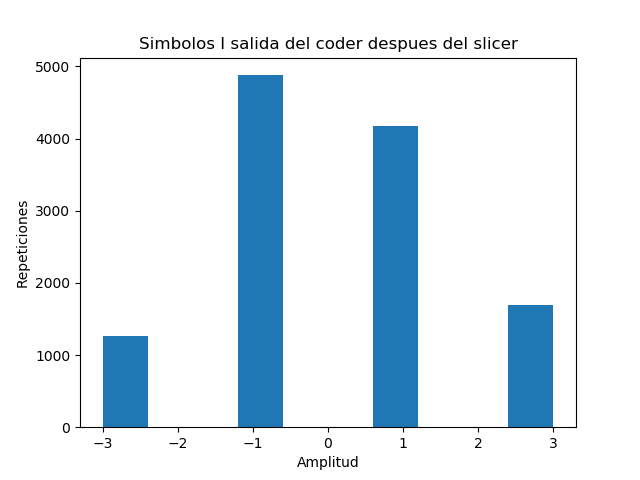
\includegraphics[width=\textwidth]{Graficos/I_symbols_slicer.png}
    \end{figure}
    \end{column}
\end{columns}
\end{frame}

\begin{frame}
  \frametitle{\textbf{Resultados obtenidos}}
   \framesubtitle{\secname : \subsecname}
   Símbolos codificados, $P_{(x=0)}=0.25$
    \vspace{-0.3cm}

\begin{columns}
    \begin{column}{0.48\linewidth}  
    \begin{figure}
        \centering
    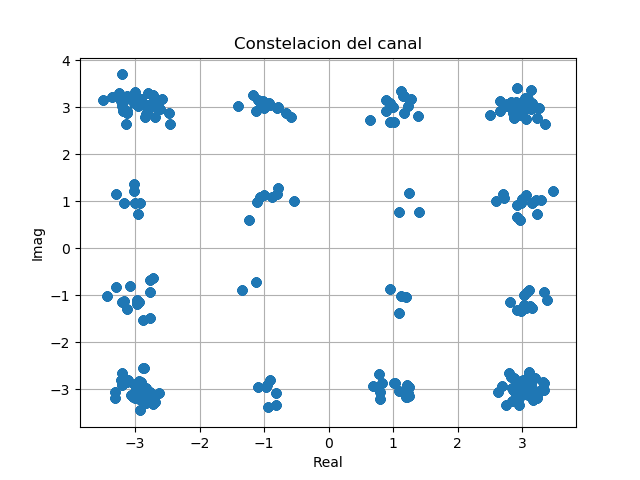
\includegraphics[width=\textwidth]{Graficos/Channel_Constelation_3.png}%
    \end{figure}
    \end{column}

    \begin{column}{0.48\linewidth}
    \begin{figure}
        \centering
    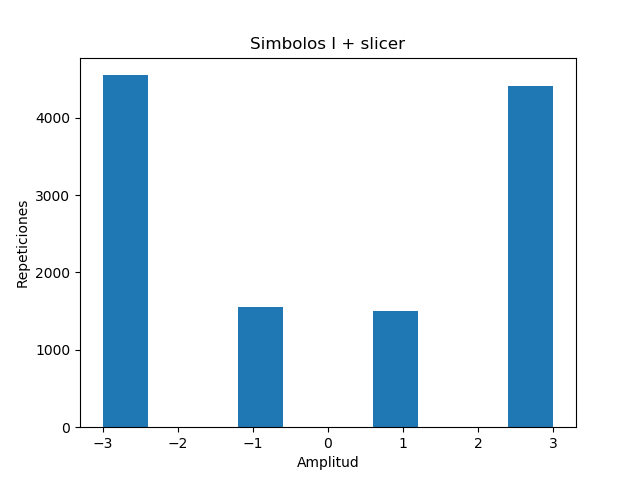
\includegraphics[width=\textwidth]{Graficos/I_symbols_slicer_3.png}
    \end{figure}
    \end{column}
\end{columns}
\end{frame}

